\documentclass[12pt]{article}
\usepackage[table]{xcolor}
\usepackage[shortlabels]{enumitem}
\usepackage{tabularx,xltabular}
\usepackage{graphicx}
\usepackage{adjustbox}
\usepackage{hyperref}
\usepackage{verbatim}
\usepackage{geometry}
\usepackage{scalerel}
\usepackage{ulem}
\usepackage[official]{eurosym}
\usepackage{tikz}
\usetikzlibrary{arrows,backgrounds,calc,decorations.markings,patterns,3d,positioning,fit,angles, quotes}
\usepackage{pgfplots}
\usepackage{circuitikz}
\pgfplotsset{compat = newest}
\usetikzlibrary{fit}
\newcommand\addvmargin[1]{
\usetikzlibrary{arrows}
\node[fit=(current bounding box),inner ysep=#1,inner xsep=0]{};}
\usepackage{cancel}
\usepackage{fontspec}
\usepackage{array}  
\geometry{a4paper, top=2cm, left=2cm, right=2cm, bottom=2cm, headsep=1cm}
\usepackage{tabu}
\usepackage{pst-node}
\usepackage{colortbl}
\usepackage{array}
\setlength\parindent{0pt}
\newcolumntype{?}{!{\vrule width 1pt}}
\usepackage{makecell}
\usepackage{pbox}
\usepackage{amssymb}
\usepackage{amsmath}
\usepackage{booktabs}
\newcolumntype{L}[1]{>{\raggedright\let\newline\\\arraybackslash\hspace{0pt}}m{#1}}
\newcolumntype{C}[1]{>{\centering\let\newline\\\arraybackslash\hspace{0pt}}m{#1}}
\newcolumntype{R}[1]{>{\raggedleft\let\newline\\\arraybackslash\hspace{0pt}}m{#1}}
\def\mcirc{\mathbin{\scalerel*{\circ}{j}}}
\def\msquare{\mathord{\scalerel*{\Box}{\strut}}}
\begin{document}
\rightline{}
\centerline{{\Large }} 
\noindent \\


\tikzstyle{background grid}=[draw, black!15,step=.5cm]
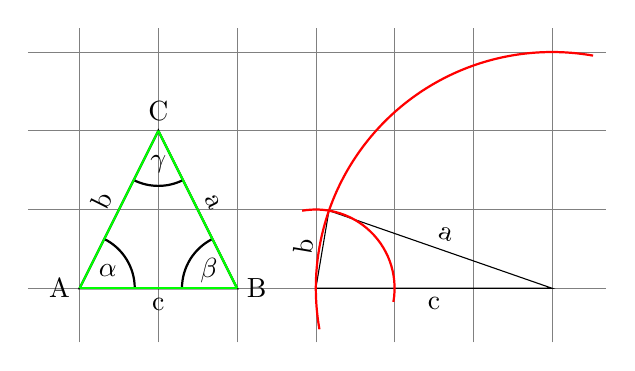
\begin{tikzpicture}[show background grid]
\coordinate (A) at (0,0);
\coordinate (B) at (0:3);
\coordinate (C) at (80.40593177313954:1);
\draw (A) -- node[below,sloped] {c} (B)   -- node[above,sloped] {a} (C)  -- node[above,sloped] {b} (A);
\draw[thick,red] ($(A)+(-10:1)$) arc (-10:100:1 cm);
\draw[thick,red] ($(B)+(80:3)$) arc (80:190:3 cm);
\draw[thick,black] (-3,0) coordinate(A) -- node[below,sloped]{c} ++(2,0) coordinate(B) -- node[above,sloped]{a} ++(-1,2) coordinate(C) -- node[above,sloped]{b} cycle; 
\node[left] at (A) {A};
\node[right] at (B) {B};
\node[above] at (C) {C};
\pic [draw,thick, black,angle radius=0.7cm, "$\alpha$"] {angle = B--A--C};
\pic [draw,thick, black,angle radius=0.7cm, "$\beta$"] {angle = C--B--A};
\pic [draw,thick, black,angle radius=0.7cm, "$\gamma$"] {angle = A--C--B};
\draw[thick,green] (B) -- (C);
\draw[thick,green] (A) -- (C);
\draw[thick,green] (A) -- (B);
\end{tikzpicture}
\end{document}